\documentclass{article}

\usepackage{graphicx}
\usepackage{amsmath}
\usepackage{courier}
\usepackage{float}
\usepackage{booktabs}
\usepackage{array}

\begin{document}

\begin{titlepage}
\begin{center}


{\huge \textbf{COS 710: Assignment II}}

\vspace{1cm}

{\Large \textbf{Genetic Programming: Transfer Learning}}

\vspace{1cm}

{\large u22498037 \\
University of Pretoria}


\vfill

\end{center}
\end{titlepage}

\tableofcontents

\newpage

\section{Running Instructions}
To run the GP, made with C++, a \texttt{makefile} is included as part of the submission. You can use the following commands in the directory to run the GP:

\begin{verbatim}
  make
  make run
\end{verbatim}

Since architectures may vary, the following can be commands can also be used to (hopefully) run the GP when \texttt{clang} is installed: 

\begin{verbatim}
  make alt
  make run
\end{verbatim}

Running this on a Macbook Air M1 with 16GB RAM took about 30 seconds per run. There is no need to run the preprocessing script again.

\section{Exploratory Data Analysis (EDA)}
To understand the data, Exploratory Data Analysis (EDA) were done to understand the relationship between the different datasets to discover how transfer learning can be applied. To determine dataset relatedness, the overlapping columns in both datasets were described by their count, mean, standard deviation, minimum and maximum values, and 25th/50th/75th percentiles. Each value in the one dataset's summary was then subtracted by their respective value in the other dataset's summary (Table \ref{tab:small_stats}). For example, with the means of each dataset, \(\mbox{mean}_{relatedness} = |\mbox{mean}_{small} - \mbox{mean}_{act}|\).

By inspecting Table \ref{tab:small_stats}, it is clear that these two datasets are identical except for the additional variables\footnote[1]{\label{note1}These variables are pgout, ppgout, pgfree, pgscan, atch, pgin, ppgin, pflt, vflt} found in \texttt{197\_cpu\_act.csv}. The transfer learning method will be discussed later in this report.

\begin{table}[h!]
  \centering
  \caption{Relatedness of overlapping variables in the respective dataset where \\ (\(\mbox{X}_{relatedness} = |\mbox{X}_{small} - \mbox{X}_{act}|\))}
  \label{tab:small_stats}
  \begin{tabular}{lrrrrrrrr}
  \toprule
   & count & mean & std & min & 25\% & 50\% & 75\% & max \\
  \midrule
  sread & 8192.00 & 0.00 & 0.00 & 0.00 & 0.00 & 0.00 & 0.00 & 0.00 \\
  freemem & 8192.00 & 0.00 & 0.00 & 0.00 & 0.00 & 0.00 & 0.00 & 0.00 \\
  wchar & 8192.00 & 0.00 & 0.00 & 0.00 & 0.00 & 0.00 & 0.00 & 0.00 \\
  fork & 8192.00 & 0.00 & 0.00 & 0.00 & 0.00 & 0.00 & 0.00 & 0.00 \\
  scall & 8192.00 & 0.00 & 0.00 & 0.00 & 0.00 & 0.00 & 0.00 & 0.00 \\
  swrite & 8192.00 & 0.00 & 0.00 & 0.00 & 0.00 & 0.00 & 0.00 & 0.00 \\
  exec & 8192.00 & 0.00 & 0.00 & 0.00 & 0.00 & 0.00 & 0.00 & 0.00 \\
  rchar & 8192.00 & 0.00 & 0.00 & 0.00 & 0.00 & 0.00 & 0.00 & 0.00 \\
  runqsz & 8192.00 & 0.00 & 0.00 & 0.00 & 0.00 & 0.00 & 0.00 & 0.00 \\
  freeswap & 8192.00 & 0.00 & 0.00 & 0.00 & 0.00 & 0.00 & 0.00 & 0.00 \\
  lread & 8192.00 & 0.00 & 0.00 & 0.00 & 0.00 & 0.00 & 0.00 & 0.00 \\
  lwrite & 8192.00 & 0.00 & 0.00 & 0.00 & 0.00 & 0.00 & 0.00 & 0.00 \\
  \hline
  target & 8192.00 & 0.00 & 0.00 & 0.00 & 0.00 & 0.00 & 0.00 & 0.00 \\
  \bottomrule
  \end{tabular}
  \end{table}

\section{Preprocessing}
\emph{To keep the report concise, only the \texttt{lread}-variable was used in the figures. The other variables followed the same pattern more or less. The data shown is also based on the \texttt{227\_cpu\_small.csv} dataset and the exact same approach was taken with the other dataset. The preprocessing script was also included, but there is no need to run it again. }

\subsection{Duplicates}
No duplicates were detected and therefore no further action were taken in this regard.

\subsection{Outliers}
During EDA, outliers across the dataset were identified. An example of the \texttt{lread}-variable is visualised as a boxplot in Figure \ref{boxplot}.

\begin{figure}[H]
  \makebox[\textwidth][c]{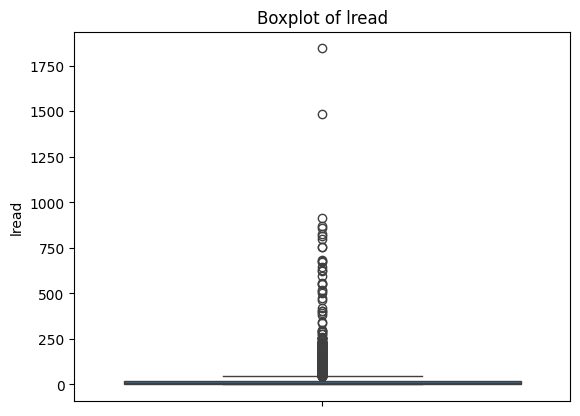
\includegraphics[width=0.5\textwidth]{assets/boxplot.png}}
  \caption{A boxplot visualising outliers of the \texttt{lread}-variable evident in the original dataset.}
  \label{boxplot}
\end{figure}

Since the dataset is of sufficient size, the entries with outliers could be removed. To remove the outlier entries, data points with a \(\pm{2}\) \(Z\)-score (an indication of how many standard deviations the point is away from the mean) were removed. Figure \ref{outlier} visualises how these outliers were removed. In practice, \(\pm{3}\) is preferred, but \(\pm{2}\) helped to better detect the outliers.

\begin{figure}[H]
  \makebox[\textwidth][c]{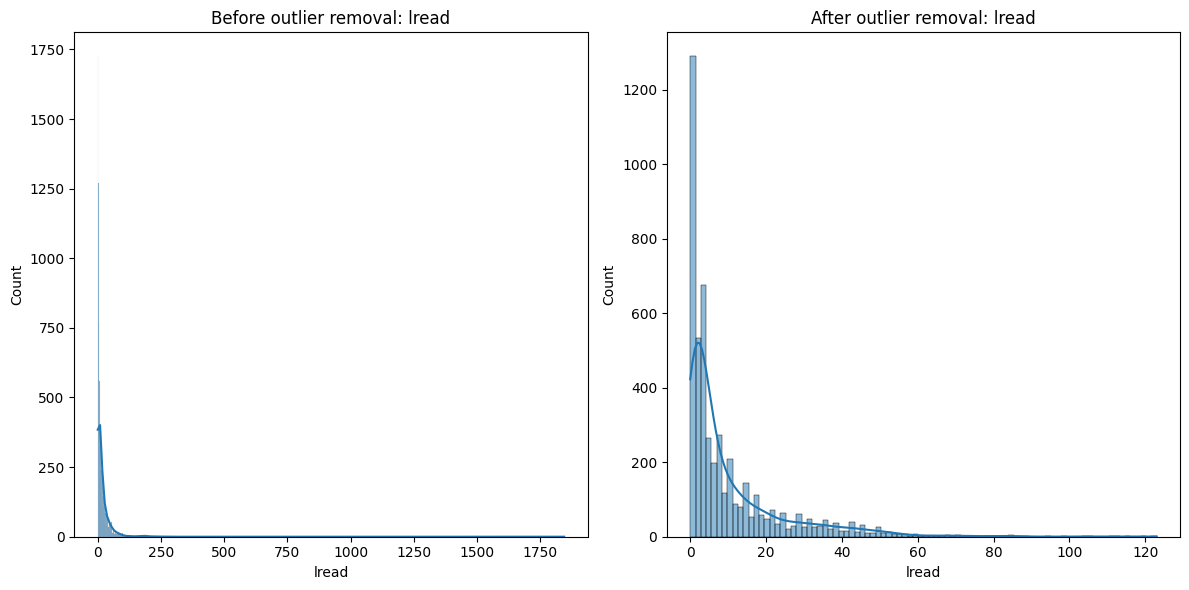
\includegraphics[width=\textwidth]{assets/outlierRemoval.png}}
  \label{outlier}
  \caption{A histogram visualising the removal outliers of the \texttt{lread}-variable when the Z-score of a data point is \(\pm{2}\).}
\end{figure}

Removing outliers helped the model to converge better due to more consistent tree outputs.

\subsection{Zero-inflated Columns}
After outlier removal, some columns still contained mostly zero values and is likely to impact the GP performance. Table \ref{zeroCols} visualises the total zero values across columns in the dataset.

\begin{table}[H]
  \centering
  \caption{Zero-inflated columns after outlier removal}
  \label{zeroCols}
  \begin{tabular}{lrr}
    \toprule
     & count & \% of total \\
    \midrule
    lread & 675 & 8.239746 \\
    lwrite & 2684 & 32.763672 \\
    scall & 0 & 0.000000 \\
    sread & 0 & 0.000000 \\
    swrite & 0 & 0.000000 \\
    fork & 21 & 0.256348 \\
    exec & 21 & 0.256348 \\
    rchar & 0 & 0.000000 \\
    wchar & 0 & 0.000000 \\
    pgout & 4878 & 59.545898 \\
    ppgout & 4878 & 59.545898 \\
    pgfree & 4869 & 59.436035 \\
    pgscan & 6448 & 78.710938 \\
    atch & 4575 & 55.847168 \\
    pgin & 1220 & 14.892578 \\
    ppgin & 1220 & 14.892578 \\
    pflt & 3 & 0.036621 \\
    vflt & 0 & 0.000000 \\
    runqsz & 0 & 0.000000 \\
    freemem & 0 & 0.000000 \\
    freeswap & 0 & 0.000000 \\
    target & 283 & 3.454590 \\
    \bottomrule
  \end{tabular}
\end{table}

To cater for this, columns were removed where more than 25\% of the values were zero. Additionally, the values where the target variable was zero was also removed.

\subsection{Skewness}
Looking at Figure \ref{targetPost}, with skewness, the model might struggle to generalise with the target variable at hand. To solve this, the Yeo Johnson transformation technique \cite{yeo2000new} was used to transform all the variables to follow an approximate normal distribution. Experiments have been done to transform only the target, but with notable performance degradation, it is not presented as part of the final solution.

\begin{figure}[H]
  \makebox[\textwidth][c]{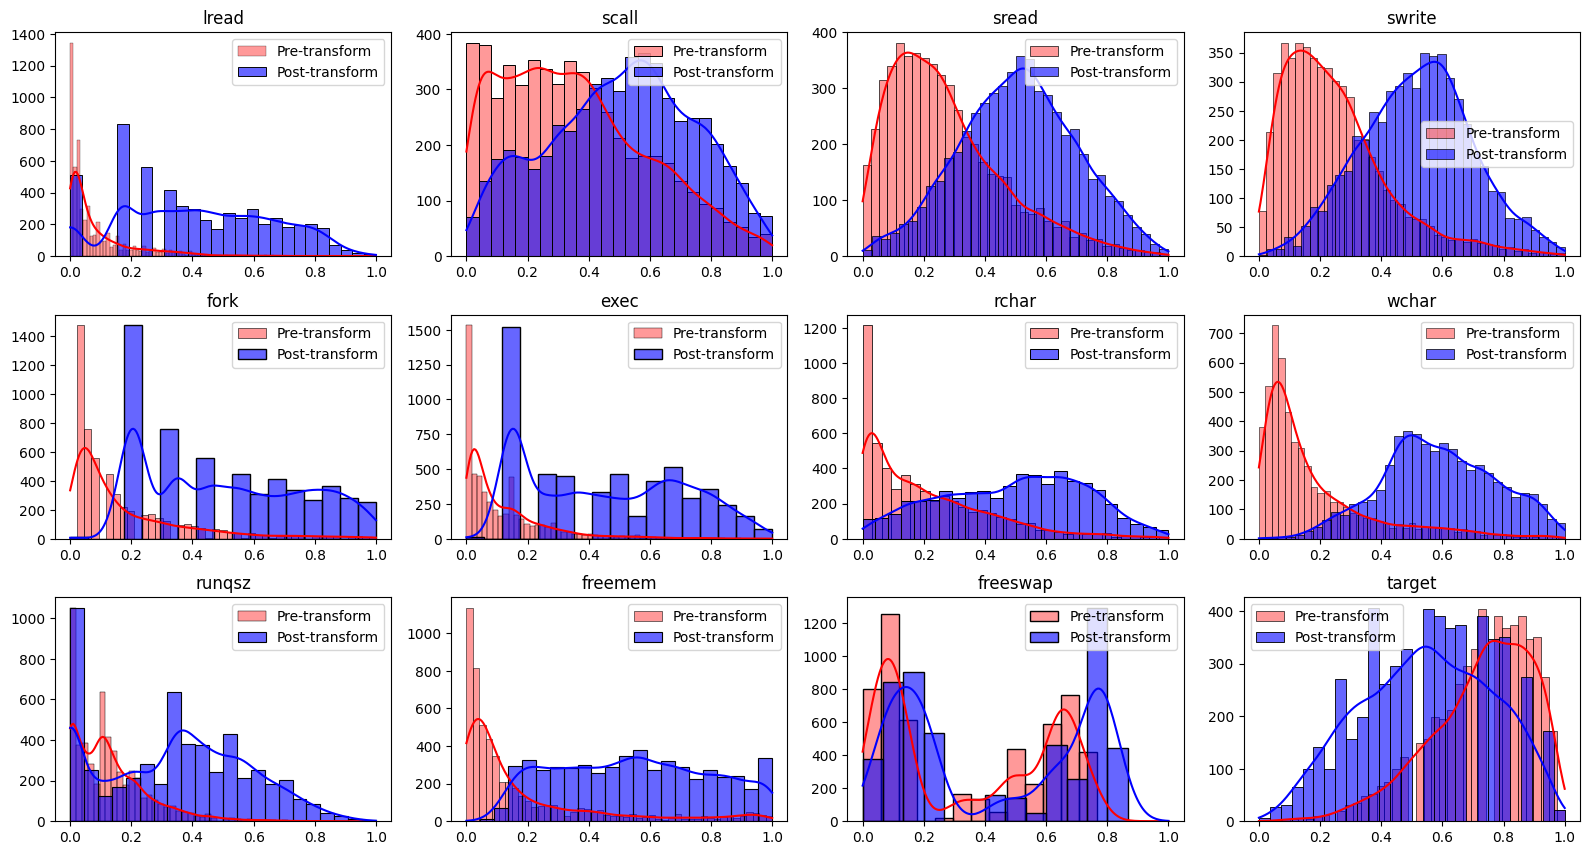
\includegraphics[width=1.25\textwidth]{assets/hist.png}}
  \caption{Histograms of all variables \textbf{before} and \textbf{after} Yeo Johnson transformation (Min-Max normalised).}
  \label{targetPost}
\end{figure}

\subsection{Column-wise Min-Max Normalisation}
The data was normalised column-wise using min-max scaling \cite{patro_2015_normalization}:
\begin{equation}\label{norm}
  X' = \frac{X-min}{max-min}
\end{equation}
This helped to preserve each column's features and its respective scale. The fitness function and some functions in the function set made use of the Sigmoid-function, and therefore normalised data was essential to the fitness function of the GP. This is described more in depth in Section \ref{fitness}, but the main takeaway is that normalisation was necessary to function with the GP's specification.

\subsection{Correlation}
After performing preprocessing, the correlation plots was used to understand how these variables interact with the target variable:

\begin{figure}[H]
  \makebox[\textwidth][c]{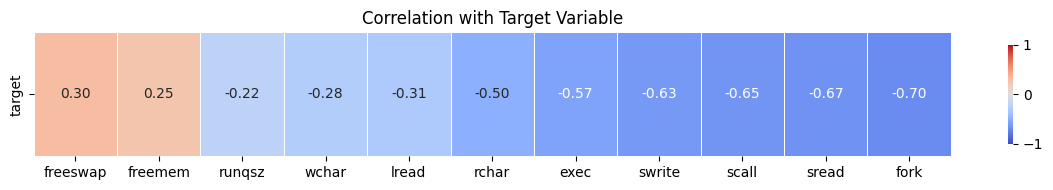
\includegraphics[width=\textwidth]{assets/corr227.png}}
  \caption{Correlation plot of the \texttt{277\_cpu\_small\_cleaned.tsv} dataset}
\end{figure}

\begin{figure}[H]
  \makebox[\textwidth][c]{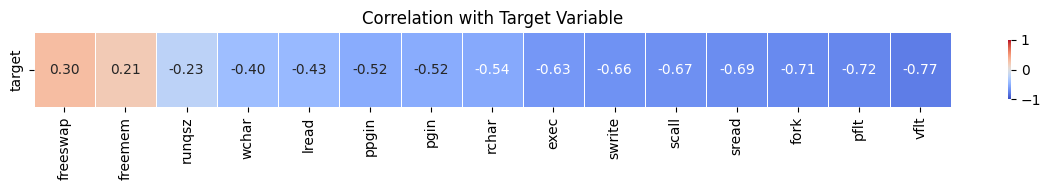
\includegraphics[width=\textwidth]{assets/corr197.png}}
  \caption{Correlation plot of the \texttt{197\_cpu\_act\_cleaned.tsv} dataset}
\end{figure}

As can be seen, the correlation plots show that most variables possess a strong negative correlation with the target variable, indicating that these variables negatively affect CPU performance. This has been noted when training the GP, but not explicitly catered for.


\section{GP Runtime Performance}
During the development of the assignment, several approaches helped to significantly improve the runtime performance of the GP. Actual performance increases were not measured, but could visibly be observed when running the code.
\subsection{Caching}
Recalculating the fitness for each individual in the population per generation is computationally intensive. To solve this, each individuals' initial fitness was cached to an array and an individual's fitness was only updated when genetic operations have been applied to the specific indidivual. This improved runtime performance significantly, although there was an initial time loss due to caching.

\subsection{Threading}
To improve the initial generation of the population and the caching mechanism, each runs' initial population were generated and cached simultaneously using multi-threading. This was eventually removed because of reproducibility problems with the seeding.

\subsection{Pass by Reference}
C++'s pass by reference ability was utilised throughout the codebase to further improve performance.

\section{GP Technical Specification}
\subsection{Transfer Learning Specification}
Since the initial and target dataset is identical except for a few additional variables in the target dataset, the last generation's population from the initial GP forms part of the target GP. These last generations converged successfully in the initial GP and is used along with the application rates and GP setup. The additional variables is added to the terminal set. For quicker convergence, the application rates were increased (described in Section \ref{GPsetup}).

With transfer learning, the attempt is to further converge the model (i.e. improve model performance), but with the introduction of additional variables. For the purpose of this assignment, transfer learning is performed in the same run as the initial GP training. The target GP will also highlight if the addition of variables makes a notable difference to the performance as well as additional generations.

The process follows a simple sequential pattern:
\begin{enumerate}
  \item The initial population is cached.
  \item The initial GP is trained on the small dataset with initial GP parameters.
  \item The best \(k\) individuals are selected.
  \item The initial population of the target GP is cached.
  \item Some GP parameters are updated in preparation for the Transfer Learning phase.
  \item The Transfer Learning phase is started and is trained on the actual dataset with updated GP parameters.
  \item The best tree is picked and tested against (unseen) testing data.
  \item The results are presented.
\end{enumerate}

\subsection{Structure}
\subsubsection{Representation}
The individuals in the population were represented as a tree. Each subtree can have up two subtrees, denoted as \texttt{left} and \texttt{right} subtrees where the functions (non-terminal nodes) were mathematical operators and the terminals (terminal nodes) were variables or real numbers. The output of this tree representation explains the CPU performance and is a symbolic regression problem. The subtree can only have one subtree when the function allows for it (e.g. '\(sin\)' only requires one variable whereas '\(+\)' requires two variables).

\subsubsection{Function and Terminal Set}
\texttt{randomTerminal()} and \texttt{randomOperator()} functions determined which terminal or operator is chosen when generating a tree. For this reason, adding functions or operators heavily impacted the GP's performance since the selection of a function/terminal follows a uniform distribution.

The GP's function and terminal set:
\begin{verbatim}
  F = {+, -, /, *, max, min, sigmoid, sin, cos, log}
  T = {double, lread, scall, sread, swrite, fork, 
        exec, rchar, wchar, runqsz, freeswap, target}
\end{verbatim}
where \texttt{double} is a random real number between -0.5 and 0.5. The \texttt{log}-function was specifically adapted to fit the normalised data. Usually the \(log\)-function functions in the range \((0,\infty)\). To cater for the ideal sigmoid domain (which is more or less between -1 and 1), the \(log\)-function was adapted to:
\[ log(x) = \begin{cases} 
      0 & x\leq -1 \\
      \frac{1}{2}log(x+1)+\frac{1}{2}  & x > -1 \\
   \end{cases}
\]

Additionally, for \emph{transfer learning}, the \texttt{pflt, pgin, ppgin, vflt} variables were added to the terminal set:

\begin{verbatim}
  T = {double, lread, lwrite, scall, sread, swrite, fork,
        exec, rchar, wchar, runqsz, freemem, freeswap, 
        pflt, pgin, ppgin, vflt}
\end{verbatim}

\subsubsection{Train/test split}
An 80\%/20\% train split was used, but the training set consisted of the first 80\% of the data, and the testing set the last 20\% of the dataset. This was applied to both the initial dataset and the target dataset. The datasets were shuffled before splitting them for training and testing.

\subsubsection{Initial Population}
The initial population was generated using a randomised grow method with \texttt{maxDepth} as a generation-specific parameter.

For each iteration, two booleans would independently determine if a left or right subtree would be further generated or not. The chance of these two booleans being true is increasingly determined by the current \texttt{maxDepth}. In the recursive function, \texttt{maxDepth} decreases as the tree grows.

\label{transferK}
For \emph{transfer learning}, the initial population consists the best \(k\) individuals from the last generation of the initial GP. \(k\) is calculated as a percentage from the population size (\(k = P_{size} * percentage\)). The remaining individuals are then generated similar to the initial GP's initial population.

To ensure the initial population is diverse enough, each individual's MSE was logged during caching. The results were as follows:

\begin{figure}[H]
  \makebox[\textwidth][c]{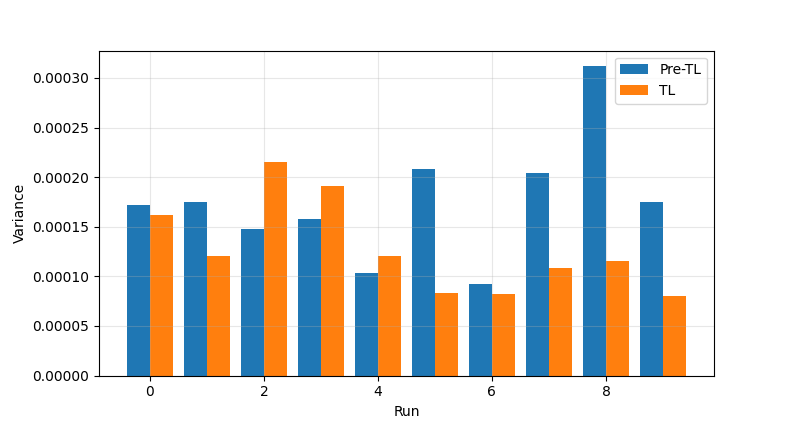
\includegraphics[width=\textwidth]{assets/diversity.png}}
  \caption{Variance of Individual Values by Run and Group}
\end{figure}

\subsubsection{Tournament Selection}
For the selection method, a tried-and-trusted tournament selection has been used. This selection method selects \(n\) random candidates to potentially apply genetic operators to. The two candidates with the best fitness is selected as parents. If the mutation operator is applied, the parent for mutation operator is randomly selected (each parent with a probability of 50\%). Intuitively, for crossover, both parents are passed as parameters, and for reproduction, the two parents are passed onto the next generation.

\subsubsection{Mutation}
For the mutation genetic operator, a mix of approaches has been followed to ensure maximum diversity. A random point in the tree is chosen, and a random subtree (possibly just a leaf node) is generated and the subtree is replaced. This ensures that both grow and shrink mutation is possible with this approach. The root node is also replacable, but because \texttt{rand() mod maxDepth} is passed as parameter, it becomes possible to penalise bigger trees, by generating a new smaller tree (i.e. the root is replaced by a smaller tree). Having a replacable root node is potentially harmful to the individual, but no notable problems have been picked up.

\subsubsection{Crossover}
The crossover operator takes a standard approach by selecting random points in each of the two parents, and then swaps them around to produce offspring. The root nodes can be swapped, but will then rather count as reproduction (the crossover application rate was adapted to account for this).

\subsubsection{Reproduction}
The selected individuals remains unchanged and is carried over to the next generation. In the codebase, the reproduction rate is calculated as \(1-C_r-M_r\) where \(C_r\) is crossover rate and \(M_r\) is mutation rate.

\subsubsection{Stopping Criteria}
For the stopping criterion, every GP run completed the full amount of generations (i.e. \texttt{maxGenerations}). No experimentation with early stopping or convergence testing has been done in this assignment. The final result were used to understand where the best convergence point were for multiple generations. Experiments with different \texttt{maxGenerations} has been done to see which one performs best.

\subsection{Fitness Function: MSE}
\label{fitness}
To evaluate the performance of the GP, Mean Squared Error (MSE) has been used as the \texttt{fitness()}-function. The reason behind this is that it can effectively capture good and bad trees and accurately represent trees' performance to improve the training process. The MSE function can be defined as follows:
\begin{equation}\label{mse}
  MSE(X) = \sum_{i=0}^{n} \frac{(f(x_i) - x_i)^2}{n}
\end{equation}

where \(X = \{x_0, x_1, ... , x_i\}\), \(n\) is the dataset size, \(f(x_i)\) is the fitness function, and \(x_i\) is the target value. In the training process, the attempt was to \textbf{minimise} \(MSE(X)\).

To prevent underflow/overflow when calculating MSE, the sigmoid function was used as a clipping function:
\begin{equation}\label{eq:sigmoid}
  sigmoid(x) = \frac{1}{1 + e^{-x}}
\end{equation}

Experiments were also done with the subtrees to clip them between -1.0 and 1.0. The subtree clipping prevents subtrees from growing large and deviating from the ability to be expressed as a value in the ideal sigmoid function range between -1.0 and 1.0 (eq. \ref{eq:sigmoid}). Since the sigmoid function was used along with normalised data, values closer to 0 were better for the model, therefore clipping between -1.0 and 1.0 helped to keep the subtrees close to the target. This was done with careful consideration.

\section{Parameters and Results}
\label{GPsetup}
The parameters were manually tuned to achieve optimal performance. A wide range of variables have been experimented with. An adjustment feature has been added to allow the GP to converge quicker and widen the search space. This might include adjustments such as an increased crossover rate. Furthermore, reasoning have been provided next to each parameter.

After fine-tuning the parameters, the following GP parameter setup is used:
\begin{itemize}
  \item Population size: 50 \emph{(Greater population size led to increased runtime with minimal performance improvements.)}
  \item Number of generations: 50 (with an additional 50 during \emph{transfer learning}) \emph{(A greater number of generations led to increased runtime with minimal performance improvements.)}
  \item Crossover rate: 0.65 (increased to 0.70 during \emph{transfer learning} to help search space exploration and convergence) \emph{(Higher crossover rates reduced convergence. A reasonably low crossover rate helped for convergence in both transfer learning (TL) and non-TL scenarios.)}
  \item Mutation rate: 0.05 (kept at 0.05 during \emph{transfer learning}) \emph{(Higher mutation rates caused the GP to struggle to find momentum towards convergence. Lower mutation rates had little impact because of the amount of generations.)}
  \item Reproduction rate: 0.30 (decreased to 0.25 during \emph{transfer learning} as a result of the increased crossover rate) \emph{(The reproduction rate was kept at a minimum to prevent stagnation and the requirement of additional generations.)}
  \item Max Depth: 4 \emph{(A small number was chosen for runtime performance reasons. Larger numbers not only affected runtime performance but also struggled to output good fitness. Larger depths did however improve divergence.)} 
  \item Tournament Size: 7 \emph{(The tournament size was made quite big to explore a big search space (14\% of the population size). Smaller tournament sizes ignored average solutions and caused overfitting.)}
  \item Percentage transferred from initial GP: 25\% (see Section \ref{transferK} for implementation details) \emph{(Larger percentages caused overfitting. Smaller percentages caused the initial population to be random.)}
  \item Run \(n\)'s seed \(i\) is \(i = n-1\). \emph{(This remained unchanged from the start.)}
\end{itemize}

Across 10 runs and a total of 1000 generations, the GP yielded the following empirical application rates:
\begin{itemize}
  \item Mutation: 66 (6.47\%)
  \item Crossover: 755 (74.02\%)
  \item Reproduction: 179 (17.55\%)
\end{itemize}

\begin{table}[htbp]
\centering
\begin{tabular}{ccc}
\hline
\multicolumn{3}{l}{\textbf{Training Statistics}} \\
\hline
\multicolumn{2}{l}{Average Best Training MSE:} & \multicolumn{1}{l}{0.0833411} \\
\multicolumn{2}{l}{Average Best Training TL MSE:} & \multicolumn{1}{l}{0.0687898} \\
\multicolumn{2}{l}{Average Fitness Improvement:} & \multicolumn{1}{l}{0.0145513} \\
\multicolumn{2}{l}{Average Duration per run:} & \multicolumn{1}{l}{32.0713 seconds (Total: 320.713 seconds)} \\
\multicolumn{2}{l}{Average TL Duration:} & \multicolumn{1}{l}{16.17 seconds (Total: 161.7 seconds)} \\
\hline
\end{tabular}
\caption{Experimental Results Summary based on \textbf{Training Data}.}
\label{timing}
\end{table}

\begin{table}[H]
\centering
\resizebox{\textwidth}{!}{
\begin{tabular}{lrrrr|rrrr}
\toprule
& \multicolumn{4}{c|}{\textbf{Initial GP}} & \multicolumn{4}{c}{\textbf{Target GP (TL)}} \\
Run & Mean & Min & Max & Std & Mean & Min & Max & Std \\
\midrule
0 & 0.048105 & 0.044452 & 0.087250 & 0.007473 & 0.044467 & 0.044452 & 0.044578 & 0.000042 \\
1 & 0.047396 & 0.044287 & 0.076577 & 0.004170 & 0.044287 & 0.044287 & 0.044287 & 0.000000 \\
2 & 0.046404 & 0.044014 & 0.054520 & 0.001198 & 0.044020 & 0.044014 & 0.044314 & 0.000043 \\
3 & 0.047545 & 0.043557 & 0.077691 & 0.004849 & 0.043734 & 0.043557 & 0.044522 & 0.000378 \\
4 & 0.047336 & 0.044571 & 0.086145 & 0.006841 & 0.044619 & 0.044571 & 0.044868 & 0.000111 \\
5 & 0.047844 & 0.043808 & 0.125116 & 0.010916 & 0.043808 & 0.043808 & 0.043808 & 0.000000 \\
6 & 0.047807 & 0.044615 & 0.076817 & 0.004724 & 0.044652 & 0.044615 & 0.044716 & 0.000049 \\
7 & 0.048026 & 0.044309 & 0.104673 & 0.007978 & 0.044215 & 0.043846 & 0.044309 & 0.000189 \\
8 & 0.046997 & 0.044361 & 0.080928 & 0.005577 & 0.044361 & 0.044361 & 0.044361 & 0.000000 \\
9 & 0.048368 & 0.044466 & 0.119489 & 0.010520 & 0.044466 & 0.044466 & 0.044466 & 0.000000 \\
\hline\hline
Avg & 0.047583 & 0.044244 & 0.088921 & 0.006425 & 0.044263 & 0.044198 & 0.044423 & 0.000081 \\
\bottomrule
\end{tabular}}
\caption{Comparison of Best Tree Fitness (MSE) Statistics Before and After Transfer Learning based on \textbf{Test Data}.}
\label{table:combined_stats}
\end{table}

\section{Discussion}
After initial training, the results were mostly consistent and converged to a low MSE. There were the runs where the MSE were a bit too high for preference, but in general the GP performed well. A bad initial GP also didn't mean that the target GP (with TL) would also turn out bad, although that did make it more difficult to converge to a low test MSE value.

Furthermore, preprocessing really made a big difference as the quote says: "The success of a machine learning model is directly proportional to the quality of the data you feed it.". As evident in the report, a large amount of preprocessing has been done and this turned out to be extremely beneficial.

There were some inconsistencies in the runs later to achieve reproducible fitness across multiple runs especially after increasing the diversity (by increasing variables such as \texttt{maxDepth}). This most likely had to do with the variety of bigger trees as opposed to smaller ones. This was regarded as a tradeoff: diversity with bad fitness or reproducible fitness with bad diversity.

In terms of runtime performance, the optimisation helped to swiftly iterate on different parameters and therefore no automated parameter fine-tuning has been done.

Transfer learning was regarded as a separate training process, although it is done in the same run for demonstration purposes. Ideally, the initial GP would be saved as a model (or just the best \(k\) individuals from the last generation) and transfer learning would be directly applied to it.

Clipping the function with both the sigmoid function and intermediary min-max clipping discussed in Section \ref{fitness} also massively helped the model converge. Using the fact that the values are normalised and ensuring the tree outputs normalised values not only helped to converge the GP, but also to have a strong population of individuals that are canditates to be the best tree. There will be bad trees as well, and therefore, as mentioned earlier on, the clipping was done with careful consideration.

In general, over the 10 runs, the results were satisfactory as seen in Table \ref{timing}, showing good MSE on the normalised training dataset. Table \ref{table:combined_stats} exhibits the MSE fitness statistics before and after TL based on the test data. It is evident by looking at the standard deviation of the initial GP that a lot of exploitation of the best individuals have been done, whereas with the target GP the solution remained much more stable throughout the run. It can also be observed that the initial GP had a lower mean than the target GP, explaining that the GP further converged using the target dataset. From a logical perspective, it makes sense that the target GP will have to perform better, especially if the target domain is basically the initial domain that is "enhanced" with more variables.

By comparing Table \ref{table:combined_stats} and Table \ref{timing}, it is also clear that the GP solution didn't experience overfitting or underfitting (the MSE values are close to each other). If time allowed, possible explorations could include more advanced preprocessing, adding even more functions to the function set and experimenting with other genetic operators. Nonetheless, the results in this report is regarded as sufficient and the GP is able adequately predict CPU performance.

\bibliographystyle{IEEEtran}
\bibliography{COS710A1}

\end{document}
